\subsection{Team meetings}	
\subsubsection{29.09.14}

\begin{enumerate}
	\item The time of beginning and ending of the meeting: 18:00 - 21:30
	\item Purposes of the meeting:
	\begin{enumerate}
	  \item Discuss the rules of FTC Cascade Effect.
	  
	  \item Discuss the main aspests of robot's construction.
	  
      \item Elaborate strategy of our team's play. 
    \end{enumerate}
	\item Work, that has been done
	\begin{enumerate}
	  \item  Was discussed in part 2 of rules.
	  
	  \item During the discussion of construction of robot there have been several ideas: 
	  \begin{enumerate}
	    \item Dimensions of the robot:
	    \begin{enumerate}
	      \item Body of robot must be compact enough. Body and gripper for balls must fit at the regulated dimentions.
	      
	      \item Robot must be compact not to bother alliance partner.
	      
	      \item Body of robot shouldn't be too small,otherwise t will be unstable when the lift is raised to maximum height (120cm)
	      
	    \end{enumerate}
	    
	    \item Wheel base:
	    \begin{enumerate}
	      \item Construction with four standard wheels from set Tetrix. This system can move in a straight line and turn on the spot very good. A minor defect of this construction is that when the robot is turning wheels jump and robot shakes.  
	      
	      \item Construction with two caterpillars. This construction's advantage is that it can move in a straight line and turn on the spot. The disadvantage of this system is that caterpillar can get off. Otherwise there is no caterpillars in Tetrix set so we have to make to their ourself.  
	      
	      \item Construction with four omni wheels from Tetrix set fixed at angle of 45 degrees to the body of robot. The advantage of this construction is that it can move to any direction and can turn very fast but it move badly in a straight line. That could adversely affect the Autonomous period.
	      
	      \item Construction with four mechanum wheels that fixed as standard wheels. Advantages: good moving in a straight direction, fast turning, possibility of moving to any direction. Disadvantages:  they have low accuracy when turning we have to buy this wheels separately from the set.
	      
	      \begin{figure}[h]
	      	\begin{minipage}[h]{0.165\linewidth}
	      		\center  
	      	\end{minipage}
	      	\begin{minipage}[h]{0.6\linewidth}
	          \center{\includegraphics[scale=0.3]{days/29.09.14/images/01}}
	          \caption{Ideas of wheel base: 1)Construction with four standard wheels 2)Construction with two caterpillars 3) Construction with four omny wheels from Tetrix set 4)Construction with four mechanum wheels}
	        \end{minipage}
	      \end{figure}
	      
	    \end{enumerate}
	    
	    \item System of control of balls:
	    \begin{enumerate}
	      \item Basket for balls is fixed to the system of retractable slats that are interconnected  with help of servomotors. Advantages: the absence of a line that can tear. Disadvantages: the complexity and low reliability.	
	      
	      \item Basket for balls is fixed to system of retractable slats that are fixed to body of robot. DC-motors reel up the line and extract the lift. Advantages: this construction is simple and reliable (except the line). Disadvantages: line can tear.
	      
	      \item Basket for balls is fixed to system of retractable slats that are fixed to DC motor so it can rotate slats in the vertical plane. Advantages: opportunity of extracting in horizontal position that relieves the load from the line. Disadvantages: line can tear.
	      \begin{figure}[H]
	      	\begin{minipage}[h]{0.2\linewidth}
	      		\center  
	      	\end{minipage}
	      	\begin{minipage}[h]{0.6\linewidth}
	      		\center{\includegraphics[scale=0.3]{days/29.09.14/images/02}}
	      		\caption{Ideas of the lift 1)Construction №1 2)Construction with stationary slats 3) Construction with slats that fixed to DC motor}
	      	\end{minipage}
	      \end{figure}
	      
	    \end{enumerate}
	    
	    \item System of fixing the moving basket (for more accurate throwing of balls to basket and for moving it):
	    \begin{enumerate}
	      \item П-shaped gripper with two servomotors fix basket between the beams. Servomotors are located at DC motor that can rotate them in vertical plane. Advantages: opportunity of raising basket. Disadvantages: takes a lot of space.
	      
          \item The hooks that can capture basket for small holes in it's base are used in the same gripper. Advantages: more compact than previous variant. Disadvantages: it could be difficult to get the hooks into the holes
			\begin{figure}[H]
				\begin{minipage}[h]{0.2\linewidth}
					\center  
				\end{minipage}
				\begin{minipage}[h]{0.6\linewidth}
					\center{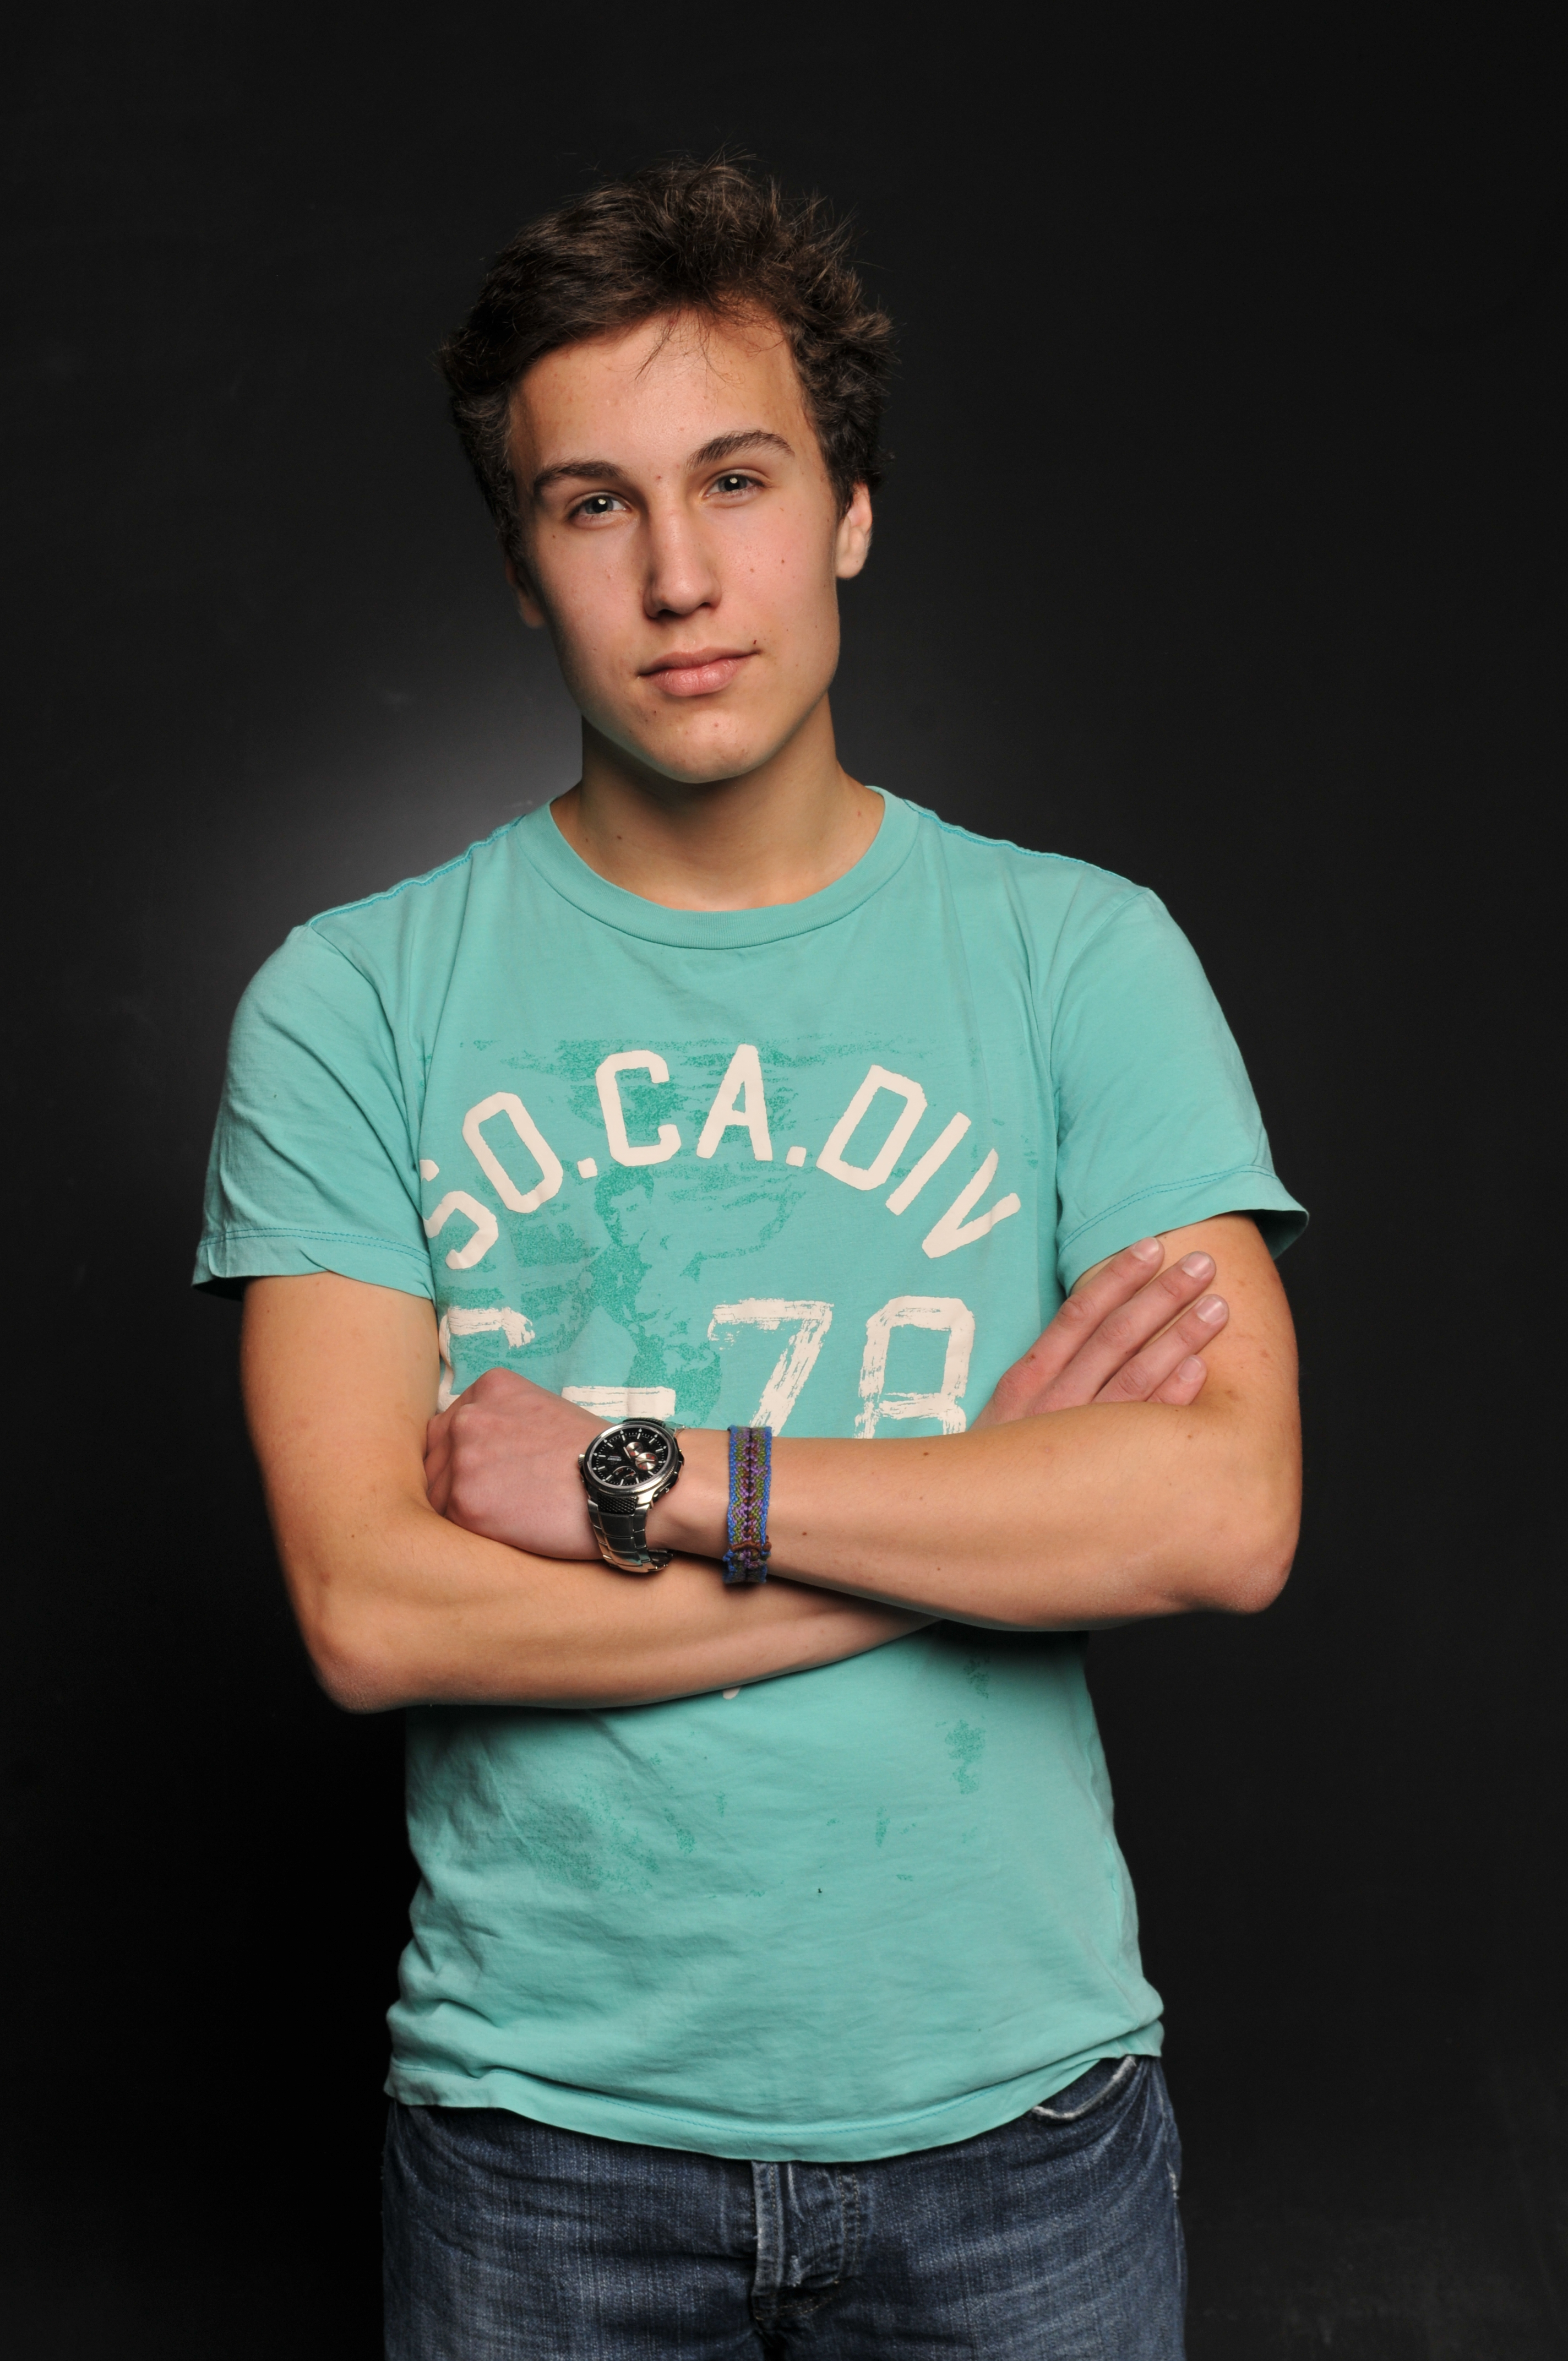
\includegraphics[scale=0.25]{days/29.09.14/images/03}}
          		\caption{Ideas of fixing of moving baskets: 1)Gripper shaped П 2)Gripper with hooks}
				\end{minipage}
			\end{figure}
          
        \end{enumerate}
      \end{enumerate}
    \end{enumerate}
    
	\item Results: 
	\begin{enumerate}
	  \item As the result of discussion were generated ideas that described in sections "Concept of robot", "Strategy" and "Planned steps for creating of the robot".      
    \end{enumerate}
    
	\item Tasks for the next meetings:
	\begin{enumerate}
	  \item To choose the wheels base.
	  
	  \item To choose the optimal sizes of robot.
	  
	  \item To choose the best system of control of balls.
	  
	  \item To choose the most effective way of fixing of moving basket.
	  
    \end{enumerate}
\end{enumerate}
\fillpage


